\section{Verteilte Systeme}

\begin{definition}{Verteiltes System}
Ein Netzwerk aus autonomen Computern und Softwarekomponenten:
\begin{itemize}
    \item Unabhängige Knoten und Komponenten
    \item Netzwerkverbindung
    \item Erscheint dem Benutzer wie ein einzelnes, kohärentes System
\end{itemize}
\end{definition}

\begin{concept}{Charakteristika verteilter Systeme}
Typische Merkmale moderner verteilter Systeme:
\begin{itemize}
    \item \textbf{Skalierbarkeit:} Oft sehr große Systeme
    \item \textbf{Datenorientierung:} Zentrale Datenbanken
    \item \textbf{Interaktivität:} GUI und Batch-Verarbeitung
    \item \textbf{Nebenläufigkeit:} Parallele Benutzerinteraktionen
    \item \textbf{Konsistenz:} Hohe Anforderungen an Datenkonsistenz
\end{itemize}
\end{concept}

\subsection{Architekturmodelle}

\begin{definition}{Architekturmodelle}
Heute finden vor allem folgende Architekturmodelle ihren Einsatz:

\textbf{1. Client/Server}
\begin{itemize}
    \item Kurzlebiger Client-Prozess kommuniziert mit langlebigem Server-Prozess
    \item Beispiel: Web-Applikation
\end{itemize}

\textbf{2. Peer-to-Peer}
\begin{itemize}
    \item Gleichberechtigte Peer-Prozesse
    \item Informationsaustausch nur bei Bedarf
    \item Beispiel: Blockchain
\end{itemize}

\textbf{3. Event Systems} (Publish-Subscribe)
\begin{itemize}
    \item Event-Sources-Prozesse und Event-Sinks-Prozesse
    \item Asynchroner Informationsaustausch
    \item Beispiel: E-Mail-System
\end{itemize}

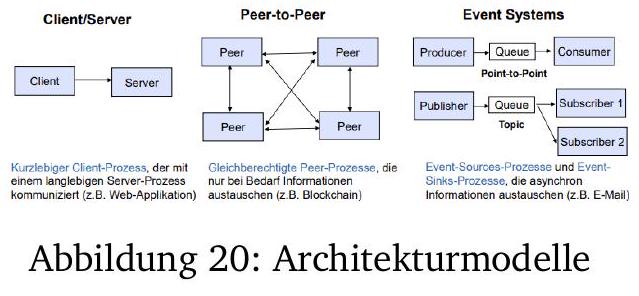
\includegraphics[width=\linewidth]{images/2024_12_29_0d1d7b5551ea1b4b41bdg-18}
\end{definition}

\subsection{Kommunikation und Middleware}

\begin{concept}{Grundlegende Konzepte}
\textbf{1. Kommunikation:}
\begin{itemize}
    \item Remote Procedure Calls (RPC)
    \item Message Queuing
    \item Publish-Subscribe-Systeme
\end{itemize}

\textbf{2. Fehlertoleranz:}
\begin{itemize}
    \item Replikation von Komponenten
    \item Failover-Mechanismen
    \item Fehlererkennung und -behandlung
\end{itemize}

\textbf{3. Fehlersemantik:}
\begin{itemize}
    \item Konsistenzgarantien
    \item Recovery-Verfahren
    \item Kompensationsmechanismen
\end{itemize}
\end{concept}

\begin{definition}{Kommunikationsmodelle}
\textbf{1. Synchrone Kommunikation}
\begin{itemize}
    \item Synchroner entfernter Dienstaufruf → blockierend
    \item Sender wartet auf Ergebnis
    \item Typisch für Request-Response Pattern
\end{itemize}

\textbf{2. Asynchrone Kommunikation}
\begin{itemize}
    \item Asynchroner entfernter Serviceaufruf → nicht blockierend
    \item Sender kann direkt weitermachen
    \item Senden und Empfangen zeitlich versetzt
\end{itemize}
\end{definition}

\begin{definition}{Middleware}
Middleware ist eine Softwareschicht, die standardisierte Dienste über ein API bereitstellt:

\textbf{Middleware-Kategorien:}
\begin{itemize}
    \item \textbf{Anwendungsorientiert:}
    \begin{itemize}
        \item Java Enterprise Edition (Jakarta EE)
        \item Spring-Framework
    \end{itemize}
    \item \textbf{Kommunikationsorientiert:}
    \begin{itemize}
        \item RPC, RMI, REST, WebSocket
    \end{itemize}
    \item \textbf{Nachrichtenorientiert:}
    \begin{itemize}
        \item Message Oriented Middleware (MOM)
        \item Java Messaging Service (JMS)
    \end{itemize}
\end{itemize}
\end{definition}

\subsection{Design und Implementation}

\begin{KR}{Entwurf verteilter Systeme}
\textbf{1. Systemanalyse}
\begin{itemize}
    \item Anforderungen identifizieren
    \item Verteilungsaspekte analysieren
    \item Konsistenzanforderungen definieren
\end{itemize}

\textbf{2. Architekturentscheidungen}
\begin{itemize}
    \item Architekturstil wählen
    \item Kommunikationsmuster festlegen
    \item Fehlertoleranzstrategie definieren
\end{itemize}

\textbf{3. Technische Maßnahmen}
\begin{itemize}
    \item Middleware evaluieren
    \item Protokolle bestimmen
    \item Werkzeuge auswählen
\end{itemize}
\end{KR}

\begin{KR}{Verteilungsprobleme analysieren}
\textbf{1. Probleme identifizieren}
\begin{itemize}
    \item \textbf{Netzwerk:} Latenz, Bandbreite, Ausfälle
    \item \textbf{Daten:} Konsistenz, Replikation
    \item \textbf{System:} Skalierung, Verfügbarkeit
\end{itemize}

\textbf{2. Lösungsstrategien}
\begin{itemize}
    \item \textbf{Netzwerk:} Caching, Compression
    \item \textbf{Daten:} Eventual Consistency, Master-Slave Replikation
    \item \textbf{System:} Load Balancing, Service Discovery
\end{itemize}
\end{KR}

%todo: Add examples for:
% - Client-Server communication
% - Event-based system
% - Load balancing setup
% - Error handling strategies